\documentclass[10pt]{article}
\usepackage[margin=0.72in]{geometry}
\usepackage[T1]{fontenc}
\usepackage{amsmath,amssymb,amsthm,mathtools,booktabs,array,microtype}
\usepackage{enumitem}
\usepackage{placeins}
\usepackage{graphicx}
\usepackage{tabularx}
\usepackage{xcolor}
\usepackage{hyperref}
\setlength{\parskip}{2.5pt}
\setlength{\parindent}{1.2em}
\setlist{nosep,leftmargin=1.6em}
\newtheorem{theorem}{Theorem}[section]
\newtheorem{proposition}[theorem]{Proposition}
\newtheorem{lemma}[theorem]{Lemma}
\newtheorem{corollary}[theorem]{Corollary}
\theoremstyle{definition}
\newtheorem{definition}[theorem]{Definition}
\newtheorem{example}[theorem]{Example}
\newtheorem{remark}[theorem]{Remark}

\newcommand{\statusline}{Preprint, version 0.5}

\hypersetup{
  colorlinks=true,
  linkcolor=black,
  citecolor=black,
  urlcolor=blue,
  pdftitle={Sharp Optimization-Robustness Envelopes for Classical Synthetic Control},
  pdfauthor={Maarten Linus Herrmann},
  pdfsubject={Version 0.5, 27 October 2026; exact bilevel geometry and certificates},
  pdfkeywords={synthetic control, bilevel optimization, robustness, exact computation, sensitivity analysis}
}
\newcommand{\R}{\mathbb R}
\newcommand{\Q}{\mathbb Q}
\newcommand{\DeltaJ}{\Delta_J}
\newcommand{\DeltaK}{\Delta_K}
\newcommand{\cG}{\mathcal G}
\newcommand{\cA}{\mathcal A}
\newcommand{\cS}{\mathcal S}
\newcommand{\conv}{\operatorname{conv}}
\newcommand{\relint}{\operatorname{relint}}
\newcommand{\argmin}{\operatorname*{arg\,min}}
\newcommand{\argmax}{\operatorname*{arg\,max}}
\newcommand{\eps}{\varepsilon}
\newcommand{\ones}{\mathbf 1}
\newcommand{\code}[1]{\texttt{#1}}

\title{Sharp Optimization-Robustness Envelopes for\\
Classical Synthetic Control}
\author{Maarten Linus Herrmann\\
\small Erasmus School of Economics\\
\small Erasmus University Rotterdam\\
\small Rotterdam, the Netherlands\\
\small\href{https://orcid.org/0009-0005-8721-6588}{ORCID 0009-0005-8721-6588}}
\date{\statusline\\27 October 2026}

\usepackage{xurl}
\begin{document}
\maketitle
\vspace{-1.25em}

\begin{abstract}
The data-driven Abadie--Diamond--Hainmueller synthetic control is an optimistic
bilevel procedure: predictor weights index a set-valued donor-weight problem,
and pre-treatment outcome loss selects among its solutions.  We define sharp
post-treatment effect envelopes over every global or outer-loss-near-global
solution admitted by that same procedure.  These deterministic envelopes are
not confidence intervals.

For rational data, we prove that the donor-weight projection of the complete
lower solution graph is a finite union of rational polytopes indexed by
coordinate matches and compatible donor-hull face/orthant pairs.  Finite convex
quadratic and linear programs then give exact global optima, exact-optimum
effect endpoints, and separate sign-spanning and attained-zero thresholds.
Numerical solvers may discover supports, but independent rational KKT and
duality checks accept certificates.  Exact synthetic examples show that an
envelope can span zero before any zero effect is attainable, which is
impossible for a convex donor-weight class under an affine effect.  For the declared Basque and California Proposition 99 designs, certified
results remain negative through the reported loss gaps. These are procedural
checks, not replications of published scalar effects.  A supporting extension gives a sufficient exact
certificate system for standardized positive predictor-weight floors.  The
contribution is an SCM-specific finite-graph specialization and certified
effect image; reliable point solvers and effect intervals over other convex
weight classes are established prior work.
\end{abstract}

\section{Introduction}

Synthetic control constructs a counterfactual for one treated unit as a convex
combination of untreated donors.  In the classical data-driven procedure,
donor weights minimize a predictor discrepancy under a diagonal matrix of
predictor weights, while the predictor weights are chosen to minimize a
pre-treatment outcome loss~\cite{abadie2003,abadie2010,abadie2011}.  This
nested construction is widely implemented by \textsf{Synth}, but it is not an
ordinary convex program in the two sets of weights.  Reliable computation has
long been a concern~\cite{becker2018,albalate2021}; Malo et al.~\cite{malo2024}
formalize the optimistic bilevel problem, establish general hardness, and give
a convergent point-optimization procedure.

Point computation leaves a different question unresolved.  Suppose the same
declared ADH fitting problem admits several global solutions, or several
solutions whose validation loss differs by no more than a substantively small
amount.  Do they imply the same post-treatment effect?  A numerical optimizer
returns one selection and cannot answer this question by itself.  We therefore
hold the estimator, data, donor pool, predictor transformation, and tie
convention fixed, and optimize the reported effect over the complete admissible
solution set.

For outer-loss tolerance $\eps\ge0$, write the resulting endpoints as
\[
  \underline\tau(\eps)=\min_{(v,w)\in\cA_\eps}\tau(w),\qquad
  \overline\tau(\eps)=\max_{(v,w)\in\cA_\eps}\tau(w).
\]
The interval between them is an envelope.  It need not equal the attained
effect set, because the bilevel graph can be disconnected.  We accordingly
separate the first tolerance at which endpoint signs straddle zero from the
first tolerance at which an exactly zero effect is attainable.

This question sits between computation and sensitivity analysis.  It is not a
sampling interval, prediction interval, placebo distribution, or robustness
set for causal-model misspecification.  Those remain essential but distinct
tasks~\cite{firpopossebom2018,cattaneo2021,fermanpinto2021}.  Nor is the broad
idea of an effect range over alternative weights new.  Ferguson and
Ross~\cite{fergusonross2021} bound effects over convex constrained-error
neighborhoods of one-level synthetic-control solutions, and Koo and
Guo~\cite{kooguo2026} minimize and maximize over a convex population moment
class.  Our object differs only after preserving the set-valued, finite-sample
ADH bilevel restriction.

The paper makes four contributions.

\begin{enumerate}
\item We define exact and near-optimal ADH effect envelopes, distinguish sign
spanning from attained zero, and give rational examples where the two
thresholds differ.
\item We eliminate continuous predictor weights geometrically.  The
donor-weight projection of the complete lower solution graph is a finite union
of rational polytopes.  The representation is constructive for two predictors
and supplies exact global optimization and effect certificates.
\item We separate numerical discovery from mathematical acceptance.  Floating-
point solvers nominate supports; exact rational KKT, LP duality, and Farkas
witnesses certify every reported claim.  Relaxation sandwiches give rigorous
bounds when full graph enumeration is combinatorially unrealistic.
\item We evaluate full public Basque and California designs and implement the
two closest convex prior feasible sets on the frozen Basque panel.  Both public
applications are sign-robust; exact synthetic examples, rather than a selected
empirical failure, establish the possible pathologies.
\end{enumerate}

The method complements point solvers.  It certifies global objective values and
all-solution effect claims when its exact checks close, and otherwise leaves the
instance unresolved.  It is not a general-purpose replacement for MSCMT or the
point algorithm of Malo et al.~\cite{malo2024}, and it supplies no statistical
coverage by itself.

\section{Relation to existing work}

\subsection{Classical SCM and computation}

The original synthetic-control construction and California tobacco application
are due to Abadie et al.~\cite{abadie2010}, following the Basque application of
Abadie and Gardeazabal~\cite{abadie2003}; the software implementation is
documented by Abadie et al.~\cite{abadie2011}.  Abadie~\cite{abadie2021}
provides a broad methodological review.
The classical constraints make donor weights interpretable convex
combinations, but neither convexity of the fixed-$v$ lower problem nor good
pre-treatment fit makes the joint data-driven problem easy.

Becker and Kl\"o{\ss}ner~\cite{becker2018} develop reliable inner optimization,
identify special cases, and implement MSCMT.  They show that existing packages
can return suboptimal solutions and give an LP feasibility check for a proposed
donor vector.  Albalate et al.~\cite{albalate2021} respond to bilevel
instability by changing the estimator and decoupling predictor importance from
donor weighting.  Malo et al.~\cite{malo2024} give the closest formal treatment:
they write the optimistic bilevel problem, derive corner candidates and
donor-simplex lower bounds, prove existence and hardness, and construct an
iterative algorithm converging to an optimal point.
Their California application already reports the 1980-cigarette-sales corner
solution and loss near 2.74366.  We use that design as an external benchmark;
we do not claim to rediscover the point optimizer or the package failure.

Our question begins after these contributions: rather than reliably return one
point, characterize the entire effect image of the global and objective-gap
solution sets.  The finite face/orthant representation below also gives a
structural description of every lower solution, not only an optimal sequence.

\subsection{Alternative weight sets and statistical uncertainty}

Nonunique one-level donor weights and sparsity are studied by Chen and
Li~\cite{chenli2024}; penalization and regularization can select a unique or
more stable estimator~\cite{abadielhour2021,amjad2018,doudchenko2017}.  Those are
valuable alternative procedures, but selection removes rather than reports the
ambiguity of the original ADH graph.

The closest effect-range objects are convex.  Ferguson--Ross constrained error
contains the one-level outcome-loss sublevel set after a monotone tolerance
mapping.  Koo--Guo use an infinity-norm moment class and explicitly report the
effect interval over that class.  Because an affine effect maps a convex weight
class to an interval, sign spanning and attained zero coincide in both cases.
They need not coincide on the ADH graph.

Prediction intervals~\cite{cattaneo2021}, imperfect-fit analysis
\cite{fermanpinto2021}, assignment sensitivity~\cite{firpopossebom2018}, and
implementation comparisons~\cite{pickett2026} address different uncertainty
sources.  We report the optimization envelope alongside, not instead of,
statistical and design-based uncertainty.

\subsection{Optimization geometry and claim boundary}

Weighted-sum scalarization in convex multiobjective optimization is standard
\cite{ehrgott2005}; viewing ADH as a weighted sum of squared predictor
residuals is therefore not itself a contribution.  General multicriteria
quadratic efficient sets can be curved~\cite{gohyang1996}.  Classical
multiparametric QP instead obtains affine optimizers on polyhedral critical
regions under uniqueness or active-nullspace definiteness, with projection
machinery for degeneracy~\cite{tondel2003}.  Neither framework directly gives
the donor-weight projection studied here: ADH varies the Hessian, permits a
set-valued lower solution, and then eliminates predictor weights.

This distinction is substantive rather than terminological.  A generic
parametric-QP optimal-set map need not be polyhedral~\cite{klatte1985}.
KKT/MPEC and lower-value-function reformulations are standard bilevel tools
\cite{dempe2002}, but they preserve an implicit graph rather than proving the
finite donor projection below.  The bounded primary-source audit located no
direct statement of that complete ADH projection or its certified affine-effect
image.  We accordingly claim an SCM-specific structural consequence of known
normal-cone, scalarization, and bilevel machinery, not a generic parametric-QP
theorem or universal priority.

\section{The ADH optimization-robustness object}

Fix one treated unit, $J\ge1$ donors, $K\ge1$ predictors, $T_0\ge1$
validation outcomes, and a scalar post-treatment summary.  Let $x_1\in\R^K$ and
$X_0\in\R^{K\times J}$ be treated and donor predictors; let
$z_1\in\R^{T_0}$ and $Z_0\in\R^{T_0\times J}$ be validation outcomes.  Let
\[
  \Delta_m=\{u\in\R^m:u\ge0,\ \ones'u=1\}.
\]
Predictor weights are $v\in\DeltaK$ and donor weights are $w\in\DeltaJ$.
For a declared affine post-treatment effect $\tau(w)=a-b'w$, define
\begin{align}
 Q(v,w)&=(x_1-X_0w)'\operatorname{diag}(v)(x_1-X_0w),\\
 \cS(v)&=\argmin_{u\in\DeltaJ}Q(v,u),\\
 L(w)&=T_0^{-1}\lVert z_1-Z_0w\rVert_2^2.
\end{align}

The primary graph and optimistic outer optimum are
\[
 \cG=\{(v,w)\in\DeltaK\times\DeltaJ:w\in\cS(v)\},\qquad
 L_\star=\min_{(v,w)\in\cG}L(w).
\]
For absolute tolerance $\eps\ge0$,
\[
 \cA_\eps=\{(v,w)\in\cG:L(w)\le L_\star+\eps\}.
\]
Compactness and continuity make $\cG$ and $\cA_\eps$ compact, so all endpoint
optima are attained.  Relative tolerances $L(w)\le(1+\rho)L_\star$ are reported
only when $L_\star>0$; the absolute definition remains meaningful under exact
fit.

\begin{definition}[Two breakdown thresholds]
The envelope-spanning and attained-zero thresholds are
\begin{align*}
 \eps_{\mathrm{span}}&=\inf\{\eps:\underline\tau(\eps)\le0\le
     \overline\tau(\eps)\},\\
 \eps_{0}&=\inf\{\eps:\exists(v,w)\in\cA_\eps,\ \tau(w)=0\}.
\end{align*}
Always $\eps_{\mathrm{span}}\le\eps_0$, but equality requires additional
connectedness.
\end{definition}

The graph uses the closed simplex $v_k\ge0$.  This follows the mathematical
formulation in Malo et al.~\cite{malo2024} and permits coordinate corner solutions.  A
strictly positive domain, a fixed floor $v_k\ge\delta$, or a deterministic
selector within $\cS(v)$ defines a different procedure and is analyzed
separately when relevant.

\section{Finite geometry of the projected lower solution graph}

Write the donor predictor columns as $x_j\in\Q^K$, the treated predictor as
$t\in\Q^K$, the fitted point $y(w)=\sum_jw_jx_j$, and the donor hull
$C=\conv\{x_1,\ldots,x_J\}$.  Use the outward normal cone
\[
 N_C(y)=\{q:q'(z-y)\le0\ \text{for all }z\in C\}.
\]
For a sign vector $s\in\{-1,+1\}^K$, let
$O_s=\{q:s_iq_i\ge0\ \forall i\}$.
For every nonempty face $F$ of $C$, including $C$ itself, define
\[
 N_C(F)=\{q:F\subseteq\argmax_{z\in C}q'z\}.
\]
Thus $N_C(C)$ is the orthogonal complement of the direction space of
$\operatorname{aff}(C)$ and can be nontrivial when the donor hull is
lower-dimensional.

\begin{theorem}[Finite rational-polytope donor projection]\label{thm:general}
For rational predictor data, the projection of the complete lower solution graph onto
donor weights is the finite union
\[
 \bigcup_{i=1}^K B_i^0\ \cup\!!
 \bigcup_{\substack{F\text{ nonempty face of }C,\\
                     s:\ N_C(F)\cap O_s\ne\{0\}}} B_{F,s},
\]
where
\begin{align*}
 B_i^0&=\{w\in\DeltaJ:y_i(w)=t_i\},\\
 B_{F,s}&=\{w\in\DeltaJ:y(w)\in F,\ s_i(t_i-y_i(w))\ge0\ \forall i\}.
\end{align*}
Every branch is a rational polytope.  If the validation data and effect
coefficients are also rational, the global validation optimum, exact-optimum
effect endpoints, $\eps_{\mathrm{span}}$, and $\eps_0$ reduce to finitely
many rational convex QPs and LPs, with an unattainable threshold reported as
$+\infty$.
\end{theorem}

\begin{proof}
Let $r=t-y$.  Fixed-$v$ first-order optimality for projection onto $C$ is
\[
 q=\operatorname{diag}(v)r\in N_C(y). \tag{1}
\]
If some residual $r_i=0$, then $w\in B_i^0$; conversely every point of
$B_i^0$ is lower-optimal at $v=e_i$ because its lower loss is zero.  If no
residual vanishes, $q\ne0$ because $v$ sums to one.  Choose the exposed face
$F(q)=\argmax_{z\in C}q'z$.  Optimality gives $y\in F(q)$ and
$q\in N_C(F(q))$.  The face can equal $C$ when $C$ is lower-dimensional.
Setting $s_i=\operatorname{sign}(r_i)$ gives $q\in O_s$, hence
$w\in B_{F(q),s}$.

For the reverse inclusion, take $w\in B_{F,s}$ with no zero residual and a
nonzero $q\in N_C(F)\cap O_s$.  Put
\[
 \widetilde v_i=q_i/r_i\ge0,\qquad
 v_i=\widetilde v_i/\sum_\ell\widetilde v_\ell.
\]
Then $\operatorname{diag}(v)r$ is a positive rescaling of $q$.  Since
$F\subseteq\argmax_C q'z$ and $y\in F$, it satisfies (1).  Zero residuals
return to the coordinate argument.  Rational polytope faces, normal cones,
orthants, and sign inequalities give rational branch descriptions, including
duplicate donor columns and nonunique donor representations.

On one branch $L$ is a rational convex quadratic.  Fixing the active
inequalities of any minimizer leaves a nonempty rational linear KKT system;
therefore a rational minimizer exists even for a singular branch QP.  Two
minimizers on the same branch cannot have distinct fitted validation vectors,
because their midpoint would strictly lower squared validation distance.
Different branches need not share a fitted vector.  Intersecting each globally
minimizing branch with its fitted-vector equality makes its optimizer set a
rational polytope, so affine-effect extrema are LPs.  For breakdown values,
minimize $L$ on each branch after adding $\tau\le0$, $\tau\ge0$, or $\tau=0$.
Taking finitely many branch minima proves the claim.
\end{proof}

Allowing the full face is necessary.  With donor predictors $(0,0)$ and
$(1,1)$, treated predictor $(1,0)$, and $w=(1/2,1/2)$, both residuals are
nonzero, but $v=(1/2,1/2)$ makes $w$ lower-optimal: the normal
$(1/4,-1/4)$ is orthogonal to the donor segment and exposes all of $C$.
An exact adversarial suite also covers duplicate donors, affine dependence,
constant coordinates, every treated-point and zero-residual position,
simplex-boundary predictor weights, intersecting faces, $K=1$, one donor,
singular validation QPs, and multiple minimizers.

The theorem establishes finiteness, not practical enumeration.  A full
$K=13,J=16$ Basque hull has 136 facets and 58,671 nonempty faces; a naive
proper-face/sign pass contains 480,624,640 pairs.  This is consistent with the
general hardness result of Malo et al.~\cite{malo2024}.

\subsection{Tractable special cases}

\begin{proposition}[Two donors]\label{prop:twodonor}
With two donors, write $w=(t,1-t)$.  For predictor row $k$, let
$d_k=X_{0,k1}-X_{0,k2}$ and $c_k=x_{1k}-X_{0,k2}$.  If some $d_k=0$, every
$t\in[0,1]$ is lower-attainable.  Otherwise the union of lower solutions is
\[
 D=\left[\operatorname{clamp}\left(\min_k c_k/d_k,0,1\right),
          \operatorname{clamp}\left(\max_k c_k/d_k,0,1\right)\right].
\]
The exact near-optimal effect set is an interval with rational or quadratic-
surd endpoints, and $\eps_{\mathrm{span}}=\eps_0$.
\end{proposition}

The proof writes the unconstrained lower minimizer as a convex combination of
$c_k/d_k$ with weights proportional to $v_kd_k^2$.  Validation loss is a
univariate convex quadratic on $D$ and the effect is affine.

For $K=2$ and arbitrary $J$ with a two-dimensional predictor hull, exact edge
KKT conditions partition each rational hull edge at finitely many rational
roots.  Lifting each attainable fitted segment back to donor weights gives a
finite rational-polytope graph including duplicate and interior donors.  At a
rational positive gap, effect-cutoff QPs and monotone rational bisection enclose
both sharp endpoints to any requested width.  No floating cutoff comparison is
used.

\subsection{Disconnected effect geometry}

The finite union need not be connected.  A three-donor, two-predictor rational
instance has exactly two global optimistic solutions with validation loss
$41/18$ and effects $-1/3$ and $+1/3$.  A rational perturbation makes the
negative solution uniquely global.  The positive solution enters at absolute
gap $1/1000$, so the envelope spans zero after only 0.0438 percent of optimal
loss.  No zero effect is then attainable; the first one appears at gap
$26081/81000$.  This exact example separates the ADH graph from every convex
weight class under an affine effect.

\begin{figure}[ht]
\centering
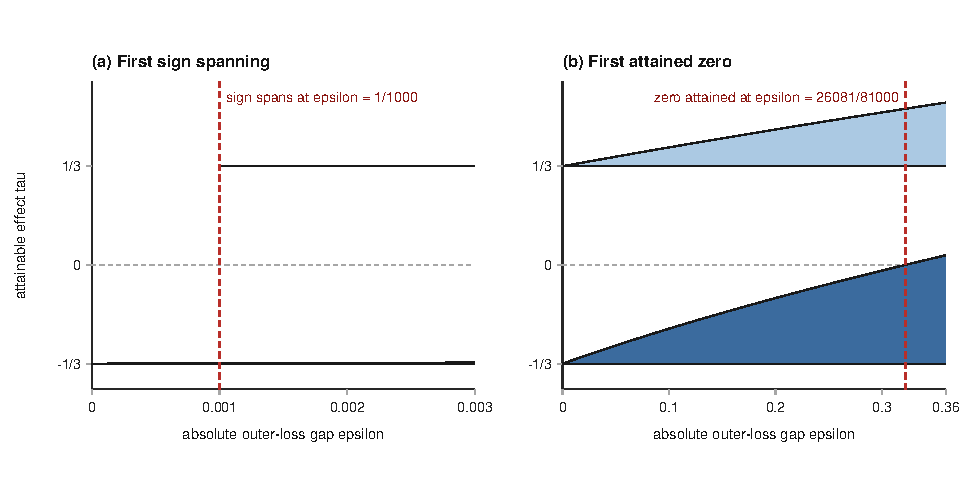
\includegraphics[width=0.92\textwidth]{figures/disconnected_effect_image.pdf}
\caption{Attainable effects in the exact rational disconnected fixture.  Each
shaded component is evaluated from its exact branch quadratic, not interpolated
between feasible weights.  Panel (a) resolves the positive component entering
at $\eps_{\mathrm{span}}=1/1000$ while the negative component remains separated
from zero.  Panel (b) shows the negative component first reaching zero at
$\eps_0=26081/81000$.}
\label{fig:disconnected}
\end{figure}
\FloatBarrier

\section{Certificates and scalable bounds}

Every constructed branch can be written as
\[
 P=\{u\ge0:Au=b\},
\]
where the first $J$ coordinates are donor weights and auxiliary coordinates
encode a fitted segment or inequality slack.  Validation optimization is a
convex least-squares QP and effect optimization is an LP.

\begin{proposition}[Exact support acceptance]\label{prop:kkt}
Suppose a numerical solver proposes positive support $S$ for a rational branch
QP.  If rational reconstruction yields a primal-feasible $u$, equality
multipliers $\lambda$, and reduced gradients satisfying
\[
 Hu-g+A'\lambda=0\ \text{on }S,\qquad
 Hu-g+A'\lambda\ge0\ \text{off }S,
\]
then $u$ is a global branch optimum.  The analogous primal-dual equalities and
inequalities certify an LP optimum.  Failure to reconstruct such a certificate
does not return an approximate claim.
\end{proposition}

This separates discovery from acceptance.  The implementation uses HiGHS and
SciPy only to nominate sparse supports.  Standard-library rational arithmetic
solves the support KKT equations, checks every equality and inequality, and
compares branch objectives exactly.  Deterministic small cases are also solved
by exhaustive rational support enumeration.

\subsection{Donor-simplex and coordinate sandwiches}

The donor simplex contains the projected bilevel graph.  Its unconstrained
validation optimum is therefore a global lower bound, and its effect-cutoff
optima are lower bounds for all ADH cutoff problems.  Any donor vector with an
exact lower-level KKT witness supplies the opposite feasible bound.  Matching
bounds close a global claim, as in the full Basque design.

Even without a general inner witness, every matchable coordinate supplies an
exact subgraph $B_i^0$ at $v=e_i$.  Let $L_R$ be the donor-simplex optimum and
$L_C$ the least validation loss among coordinate branches.  Then
\[
 L_R\le L_\star\le L_C. \tag{2}
\]
For relative tolerance $\rho$, a donor-simplex envelope at threshold
$(1+\rho)L_C$ contains the full ADH near set, while a coordinate envelope at
threshold $(1+\rho)L_R$ is contained in it.  These two calculations give
outward endpoint boxes without rounding $L_R$ and $L_C$ into equality.

\subsection{Positive predictor-weight floors}

The closed simplex admits exact coordinate matches at $v=e_k$.  Requiring
positive weights changes the procedure, and the open simplex may have an
infimum without an optimizer.  A fixed standardized floor is closed but
depends on the declared standardization.  Fix positive rational row scales
$\sigma_k^2$ and write
\[
 D(u)=\operatorname{diag}(u_k/\sigma_k^2),\qquad
 u=\delta\ones+(1-K\delta)z,\quad z\in\DeltaK,\quad 0<K\delta<1.
\]

\begin{proposition}[Sufficient exact certificate under a predictor floor]
\label{prop:floor}
Suppose the treated predictor is outside the donor hull.  For each $u$ in the
floor domain, let $y(u)$ be the unique fitted predictor point and let
$F(u)=\argmax_{x\in C}\{D(u)(t-y(u))\}'x$.  Suppose a declared finite face
family contains every $F(u)$, including the full hull if needed.  Require each
covered face to be a \emph{donor-labeled simplex}: every donor column on it is
a distinct vertex and those columns are affinely independent.  Enumerate every
nonempty subset $S$ of its donor columns.  For every $S$, construct the exact
Cramer polynomials for all support weights, all inactive-gradient inequalities,
and the outer-loss difference.  If a finite rational simplex partition proves
the outer-loss polynomial nonnegative wherever every KKT polynomial is
nonnegative, or proves that this KKT-feasible set is empty, then $c$ is a global
lower bound on floor-constrained outer loss.  An exact fixed-$u$ lower-level
witness attaining $c$ proves global optimality.
\end{proposition}

Positive $D(u)$ makes the fitted predictor point unique; donor-labeled
simpliciality makes each positive donor support rationally parameterizable.
Cramer's rule then converts lower optimality and outer loss into polynomial
sign claims on the predictor-weight simplex.  Appendix~\ref{app:floor-proof}
gives the reduction, exact coefficient rules, and adversarial exclusions.  The
result is a sufficient certificate system: certificate verification is exact,
but repeated subdivision is not asserted to terminate or find a certificate.

\section{Empirical designs}

All exact empirical claims are conditional on documented decimal exports.
Source floating precision, data construction, and causal validity are not
absorbed into mathematical $\eps$.  Table~\ref{tab:empirical} summarizes the
two retained public full designs.  Effects are treated-minus-synthetic post-period means in
the units of each outcome.

\begin{table}[ht]
\centering
\caption{Certified full-design results}\label{tab:empirical}
\small
\begin{tabularx}{\textwidth}{@{}lrrrrX@{}}
\toprule
Design & $K$ & $J$ & Global loss & Global effect & 5\% endpoint conclusion \\
\midrule
Basque & 13 & 16 & 0.004126374 & $-0.2682005$ & Both endpoint boxes negative \\
California 99 & 7 & 38 & $[2.7436616,2.7440894]$ & $[-19.5710,-19.4563]$ & Both endpoint boxes negative \\
\bottomrule
\end{tabularx}
\end{table}

\subsection{Full Basque predictor design}

The frozen design follows all 13 predictors and 16 controls in the official
\textsf{Synth} Basque example, validates on 1960--1969 GDP per capita, and
reports the mean 1970--1975 treated-minus-synthetic effect.  Direct face
enumeration is infeasible.  The donor-simplex optimizer passes an exact inner-
attainability certificate, closing global loss and effect.  The optimum effect
is $-0.2682004675$.  Sign spanning and attained zero first occur at a 109.3716
percent relative loss increase.  Certified 1 and 5 percent endpoint boxes are
fully negative.

The conventional local \textsf{Synth} run has frozen-fixture loss
0.0088647263, 114.83 percent above global, and effect $+0.0003084$.  Earlier
work already documents implementation failures in this application
\cite{becker2018}; the new result is the certified complete-graph effect and
robustness certificate, not the observation that local software can be
suboptimal.

\subsection{California Proposition 99 benchmark}

The canonical CRAN \textsf{tidysynth} design uses seven predictors, 38 control
states, and 19 validation years.  Malo et al.~\cite{malo2024} already show on source-
precision data that the global point is a corner placing all predictor weight
on 1980 cigarette sales, with loss near 2.74366; they also establish the local
\textsf{Synth} failure.  We freeze a six-decimal rational export and ask the
different question of effect robustness.

The donor-simplex/coordinate sandwich gives
\[
 L_\star\in[2.7436616405,2.7440893158],
\]
a 0.01559 percent relative-width box.  Every globally optimal effect lies in
$[-19.570993,-19.456267]$.  The certified 1 percent endpoint boxes are
$[-19.925121,-19.724084]$ and $[-19.135304,-19.050582]$; the 5 percent boxes
are $[-20.367147,-20.178410]$ and $[-18.710069,-18.484600]$.  A nonnegative or
exactly zero effect cannot enter before at least a 31,460.8 percent relative
loss increase.  The local run remains negative at $-18.7197252$, but has about
16.9 percent excess loss.  California is therefore a robustness benchmark, not
evidence that every package failure changes sign.

\subsection{Compact screen for a third public design}

We also screened a declared standard-fitting variant of the public German
reunification panel~\cite{abadie2015}.  It remained strongly sign-robust and
added no distinct phenomenon, so Appendix~\ref{app:public-screen} records its
specification and certificate status without promoting it to a third headline
application.

\section{Comparison with the closest convex feasible sets}

The comparison is at the optimization-object level, without Ferguson--Ross
placebo calibration or Koo--Guo perturbation inference.  For a one-level
simplex pre-outcome loss with optimum $L_0>0$, Ferguson--Ross constrained error
$B$ is equivalent to squared-loss slack
\[
 \eps=\bigl((1+B)^2-1\bigr)L_0.
\]
Thus fixed-$v$ one-level objective-gap envelopes are not novel.  Koo--Guo use a
sample moment polytope $\lVert\widehat\gamma-\widehat\Sigma w\rVert_\infty\le q$,
which is also convex but uses a different metric.

\begin{table}[ht]
\centering
\caption{Feasible-set distinction}\label{tab:classes}
\small
\begin{tabular}{@{}>{\raggedright\arraybackslash}p{0.15\textwidth}
                    >{\raggedright\arraybackslash}p{0.27\textwidth}
                    >{\raggedright\arraybackslash}p{0.24\textwidth}
                    >{\raggedright\arraybackslash}p{0.25\textwidth}@{}}
\toprule
Object & Weight set & Tolerance & Zero implication \\
\midrule
Ferguson--Ross & Convex one-level outcome-fit sublevel & Relative Euclidean error & Sign spanning attains zero \\
Koo--Guo & Convex simplex moment-discrepancy class & Infinity-norm moment radius & Sign spanning attains zero \\
This paper & Generally nonconvex ADH bilevel graph & Outer validation-loss gap & Spanning may precede attained zero \\
\bottomrule
\end{tabular}
\end{table}

On frozen Basque data, the Ferguson--Ross optimum and matched 1/5 percent
endpoints agree with the ADH certificate to reported precision.  At a 1 percent
relative squared-loss gap its interval is
$[-0.2948300,-0.2395807]$; at 5 percent it is
$[-0.3274251,-0.1873163]$.  This numerical agreement is not set equality: the
exact disconnected example already proves that a convex one-level class cannot
reproduce the topology of the ADH effect image in general.

The Koo--Guo class uses a third scale.  Its exact sample-moment feasibility-
floor effect on Basque is $-0.282919$.  Following the authors' default-style
radius construction, the class first spans zero at nominal
$\lambda=0.021$ on their 0.001 grid.  These results establish neither dominance
nor a tolerance conversion; the classes answer different robustness questions.

\subsection{Claim boundary}

Table~\ref{tab:claimmap} states the claim boundary explicitly.

\begin{table}[ht]
\centering
\caption{Claim boundary relative to the closest results}\label{tab:claimmap}
\small
\begin{tabularx}{\textwidth}{@{}p{0.28\textwidth}X@{}}
\toprule
Result & Relation \\
\midrule
Reliable ADH point computation & Established by Becker--Kl\"o{\ss}ner and Malo et al.; not claimed here. \\
Effects over convex weight classes & Established by Ferguson--Ross and Koo--Guo; not claimed here. \\
Scalarization, KKT, and bilevel reformulation & Established optimization machinery used here. \\
Finite complete ADH donor projection & SCM-specific structural consequence in Theorem~\ref{thm:general}; no direct statement located in the bounded audit. \\
Certified effect image over all ADH solutions & Contribution here; headline claims have independent exact replay or explicit enclosures. \\
General efficient algorithm or statistical coverage & Not claimed; enumeration can be exponential and the envelope is conditional and deterministic. \\
\bottomrule
\end{tabularx}
\end{table}

The strongest defensible category is known general machinery applied to ADH
with an SCM-specific structural consequence.  The result is neither a new
point estimate nor a blanket software-performance claim.  It is a certifiable
post-estimation diagnostic for the original set-valued procedure: after
computing or bounding $L_\star$, ask whether every solution consistent with that
fit supports the same substantive conclusion.

\section{Limitations and implications}

First, the method conditions on the specified donor pool, predictors,
preprocessing, validation window, post summary, and optimistic tie convention.
It cannot repair an invalid research design.  Second, no coverage probability
is attached to the envelope.  Sampling, assignment, and post-treatment shocks
require separate inference.  Third, the closed predictor simplex allows exact
zeros.  Becker--Kl\"o{\ss}ner motivate positive lower bounds.  Proposition
\ref{prop:floor} gives a generic exact certificate after a declared
standardization, but it is conditional on a complete donor-labeled-simplicial
face cover and successful finite subdivision.  Fixed floors are not scale
invariant, and the certificate search need not terminate.

Fourth, exact rational claims for imported data are conditional on decimal
exports.  Source binary precision and rounding uncertainty are recorded but
not conflated with $\eps$.  Fifth, finite graph structure is not polynomial
tractability.  Full enumeration is credible for small geometry; scalable
certificates rely on relaxations, sparse supports, or a small number of exact
witnesses.  A discovery failure is honest but leaves the instance unresolved.

The public-design results reject two simple narratives.  Optimization fragility
is not automatic: California remains sign-robust at enormous relative loss,
and Basque remains robust through 5 percent.  Nor is good local fit a globality
certificate: both local runs are suboptimal. Only the Basque local run has a
sign opposite to the global effect.
Reporting the objective value, predictor-weight domain, certificate status, and
effect envelope would make classical SCM analyses more transparent.

\section{Conclusion}

Classical data-driven synthetic control is a set-valued bilevel procedure.
Returning one numerical weight vector can hide both multiplicity and
near-optimal ambiguity.  We define the corresponding sharp effect envelope,
prove a finite rational-polytope representation of the donor-weight projection
of its complete lower solution graph,
and build exact certificates for global optima, endpoints, and two distinct
zero thresholds.  The theory yields closed-form and constructive algorithms in
small effective dimension and rigorous relaxation sandwiches in larger
designs.

The contribution is deliberately narrow.  Existing work already supplies
reliable point solvers, convex sensitivity intervals, and statistical
uncertainty quantification.  The missing layer is an independently replayable
answer to a procedural question: among all solutions that the declared ADH
fitting problem itself regards as global or nearly global, how much can the
reported effect change?  The public applications answer ``not at all in sign''
at the reported tolerances, while the exact rational examples establish that a
small-gap sign reversal and a gap between sign spanning and attained zero are
mathematically possible.

\section{Reproducibility}\label{sec:repro}

Frozen public fixtures, documented data provenance, exact certificates, and
independent replay scripts accompany every headline computational claim.  Discovery may
use SciPy, HiGHS, or local SCM software; acceptance uses separately implemented
rational checks.  The standard command is
\begin{center}
\code{./scripts/check\_all.sh}.
\end{center}
The optional dependency suite reruns scalable searches and public-data
reconstruction.  A manuscript-consistency check compares reported values with
certificate records, while the release audit scans tracked files, generated
PDF text and metadata, and the archive manifest for excluded material.

\section*{Acknowledgment of generative-AI assistance}

Generative AI assisted with literature organization, drafting, implementation,
and testing. A tool recorded as Luna-Max also assisted in examining proof
arguments. OpenAI GPT-6.1 Terra and GPT-6.1 Sol assisted with the October
2026 manuscript preparation. Computational claims are supported by the
exact certificates described in Section~\ref{sec:repro}; AI outputs are not
mathematical evidence.

\appendix

\section{Additional proofs}

\subsection{Existence and monotonicity}

For each $v$, $\cS(v)$ is nonempty and compact by continuity of $Q$ on
$\DeltaJ$.  If $(v_n,w_n)\in\cG$ converges to $(v,w)$, then for every
$u\in\DeltaJ$, $Q(v_n,w_n)\le Q(v_n,u)$; continuity gives
$Q(v,w)\le Q(v,u)$.  Thus $\cG$ is closed in a compact product, hence compact.
Every $\cA_\eps$ is a compact sublevel intersection.  Endpoint optima and
breakdown constrained minima are attained whenever their sign sets are
nonempty.  Nestedness of $\cA_\eps$ makes $\underline\tau$ nonincreasing and
$\overline\tau$ nondecreasing.

\subsection{Exact breakdown calculation on a branch union}

Let $D$ be the donor-weight projection of $\cG$ and define
\begin{align*}
 m_-&=\min\{L(w):w\in D,\tau(w)\le0\},\\
 m_+&=\min\{L(w):w\in D,\tau(w)\ge0\},\\
 m_0&=\min\{L(w):w\in D,\tau(w)=0\}.
\end{align*}
When the sets are nonempty,
\[
 \eps_{\mathrm{span}}=\max(m_-,m_+)-L_\star,\qquad
 \eps_0=m_0-L_\star.
\]
Each constraint is linear and therefore preserves the rational branch form.
Convex QP KKT conditions give rational minima; absent sign sets are reported as
unattainable rather than assigned an artificial finite value.

\subsection{Coordinate-sandwich endpoint logic}

Let $L_R\le L_\star\le L_C$ be (2).  The full relative-$\rho$ set has
threshold $(1+\rho)L_\star$.  Since this is no larger than
$(1+\rho)L_C$, the donor-simplex sublevel at the latter threshold is an outer
set.  Since it is no smaller than $(1+\rho)L_R$, any coordinate-branch point
below the latter threshold is a feasible inner point.  Therefore the full
lower endpoint lies between the relaxation lower endpoint and the coordinate
lower endpoint, while the full upper endpoint lies between the coordinate
upper endpoint and the relaxation upper endpoint.  Rational cutoff bisection
turns each endpoint into an outward box.

\section{Positive-floor certificate derivation}\label{app:floor-proof}

Fix a covered donor support $S=\{j_0,\ldots,j_m\}$ and use $j_0$ as base.
Let $B$ contain the predictor differences $x_{j_\ell}-x_{j_0}$ and let
$a=t-x_{j_0}$.  With $y=x_{j_0}+B\theta$, the equality-constrained inner
conditions are
\[
 A(z)\theta=b(z),\qquad
 A(z)=B'D(u(z))B,\qquad b(z)=B'D(u(z))a.
\]
Positive $D(u)$ and affine independence make $A(z)$ positive definite, so
$d_S(z)=\det A(z)>0$.  Cramer's rule gives
\[
 w_{j_\ell}(z)=\frac{n_{S\ell}(z)}{d_S(z)},\qquad
 w_{j_0}(z)=\frac{d_S(z)-\sum_{\ell=1}^m n_{S\ell}(z)}{d_S(z)}.
\]
For a singleton support, $m=0$, the empty determinant is one and the base
weight is identically one.
The complete KKT polynomial list contains every displayed weight numerator,
including the base numerator, and for every inactive donor $k$ the cleared
normal-cone inequality
\[
 -d_S(z)\,q(z)'(x_k-x_{j_0})\ge0,\qquad
 q(z)=D(u(z))(t-y(z)).
\]
The sign is fixed by the outward convention $q'(x-y)\le0$.

For validation residual numerator $E_{S,t}(z)$, exact denominator clearing gives
\[
 L(z)-c=
 \frac{P_S(z)}{T_0d_S(z)^2},\qquad
 P_S(z)=\sum_tE_{S,t}(z)^2-T_0c\,d_S(z)^2.
\]
The denominator is strictly positive.  Entries of $A$ and $b$ are homogeneous
linear forms after replacing constants by multiples of $\sum_kz_k=1$.
Consequently $d_S$ and the Cramer numerators have degree at most $m$, inactive
gradients have degree at most $m+1$, and $P_S$ has degree at most $2m$;
cancellation may lower these degrees.  Each polynomial is homogenized to its
own actual target degree before coefficient testing.

On any rational simplex cell, nonnegative degree-matched Bernstein
coefficients prove $P_S\ge0$.  A KKT cell is infeasible only if every
degree-matched coefficient of one required KKT polynomial is strictly negative,
with absent monomials treated as zero.  The latter rule is essential:
$-z_0z_1$ has one stored negative coefficient but vanishes on the boundary.
Longest-edge midpoint subdivision preserves rationality.  The verifier rebuilds
every cell and accepts only a prefix-free set of leaves that covers the root
simplex, including shared boundaries.  A missing support or uncovered cell is
an incomplete attempt, not a certificate.

The donor-labeled-simplex hypothesis cannot be weakened to geometric
simpliciality.  A segment containing a duplicate or interior donor column has
a nonunique donor fiber even when its fitted predictor point is unique; the
outer validation fit may vary across that fiber.  Enumerating every nonempty
subset handles support boundaries, while exact affine-rank checks reject
singular supports.

A rational regression fixture exercises KKT pruning.  Donor predictors are
$(0,0)$ and $(1,1)$, the treated predictor is $(1,0)$, validation values are
$0$ for the treated unit and $(0,1)$ for donors, and both declared row scales
are $1/3$.  Under $u_k\ge1/4$, the exact optimum is $1/16$ at
$u=(1/4,3/4)$ with donor weights $(3/4,1/4)$.  The first donor alone would have
outer loss zero if inner optimality were ignored, but its inactive-gradient
polynomial is strictly negative throughout the floor domain.  A separate
$(z_0-z_1)^2$ fixture requires one exact midpoint subdivision.  These fixtures
test the certificate without relying on an empirical application.

\section{Additional public benchmark screen}\label{app:public-screen}

The screened German reunification variant uses six published predictor
categories, 16 donors, 1960--1989 GDP as validation outcomes, and mean
1991--2003 GDP as the effect summary.  This declared standard-fitting variant
is not the article's two-stage cross-validation and refit.  An exact
donor-simplex/coordinate sandwich places every global effect between
$-1717.01$ and $-1256.39$ in source GDP units; zero requires at least a 560.3
percent relative loss increase, and donor-simplex outer bounds keep the 1 and
5 percent envelopes negative. The fixture and certificate document the
benchmark, but it
adds no qualitative behavior beyond the two main applications.

\section{Certificate architecture and data provenance}

The repository contains four distinct layers.

\begin{enumerate}
\item \emph{Discovery}: deterministic searches, SciPy support proposals, and
local R package runs.  These may suggest a support but prove nothing globally.
\item \emph{Acceptance}: rational LP/QP KKT checks, exact hull/face arithmetic,
and exact nonnegative-system or Farkas decisions.
\item \emph{Certificates}: JSON or text records containing exact fractions,
sparse witnesses, branch decisions, and endpoint boxes.
\item \emph{Independent replay}: verifier scripts rebuild geometry and compare
every saved claim.  Standard and optional dependency suites are separated.
\end{enumerate}

The principal commands are
\begin{center}
\code{./scripts/check\_all.sh}\qquad
\code{./scripts/check\_optional\_scalable.sh}.
\end{center}
At the paper freeze, the standard suite runs 56 tests: 50 pass and six optional
SciPy tests skip by design.  The optional suite passes six additional tests and
replays the Basque, California, closest-prior, and screened-public-design
certificates.  The positive-floor synthetic certificate is replayed with only
standard-library rational arithmetic.  When source data and repository-local R
packages are available, all committed public fixtures and local
\textsf{Synth} outputs reproduce byte-for-byte.  A release audit scans tracked
paths, public source content, PDF text, and PDF metadata before an allowlisted
archive can be built.

\begin{table}[ht]
\centering
\caption{Frozen empirical provenance}\label{tab:provenance}
\small
\begin{tabular}{@{}>{\raggedright\arraybackslash}p{0.10\textwidth}
                    >{\raggedright\arraybackslash}p{0.29\textwidth}
                    >{\raggedright\arraybackslash}p{0.23\textwidth}
                    >{\raggedright\arraybackslash}p{0.27\textwidth}@{}}
\toprule
Design & Source status & Exact-data convention & Redistribution \\
\midrule
Basque & CRAN \textsf{Synth} 1.1-10 package example & Six-decimal rational export & Package-derived fixtures committed \\
California & CRAN \textsf{tidysynth} 0.2.1 package example & Six-decimal rational export & Package-derived fixture committed \\
\bottomrule
\end{tabular}
\end{table}

All computational timing claims are descriptive.  Exact status comes from the
certificate algebra, not runtime, numerical convergence flags, or printed
decimal agreement.

\bibliographystyle{plain}
\bibliography{references}

\end{document}
